\chapter{Analyse}
De Hoofdvraag:

In dit onderzoek gaat er onderzocht worden of het S88 protocol nagebouwd kan worden met een XILINX Spartan 3E FPGA bord en de harware omschrijf taal VHDL.
\section{deelvragen}
Voor de Analyse zijn er meerdere deelvragen opgesteld,

\begin{enumerate}
	\item Hoe werkt het s88 protocol?
	\item Hoe werkt een XILINX Spartan 3E FPGA bord?
	\item Hoe kan de hardware beschrijving taal VHDL gebruikt worden op het XILINX bord?
	\item Hoe kan een schuifregister aangesloten worden op het XILINX bord?
\end{enumerate}

\subsection{Hoe werkt het s88 protocol?}
Het s88 wordt uitgelegd met behulp van de twee onderstaande afbeeldingen.
\\\\
Het Xilinx bord kan met behulp van het s88 protocol de rechter bus uitlezen. Dit gebeurt met behulp van een schuifregister.
\\\\
Met de DATA OUT poort van het Xilinx bord wordt data ingelezen. Deze is verbonden met de Q1 Out poort van het schuifregister, hiermee wordt dus informatie van het schuifregister naar het Xilinx bord overgedragen.
\\\\
Er wordt in dit onderzoek met twee termen gewerkt waarmee hetzelfde bedoelt wordt, dat zijn LATCH en Load, in de onderstaande afbeelding wordt de term LATCH gebruikt maar in het verslag wordt de term Load gebruikt.\\\\


De werking is als volgt, op het moment dat het Xilinx bord een positieve flank geeft op de CLOCK en de Load hoog is, dan zal het schuifregister de data op Ingang D inlezen. Geeft het Xilinx een positieve flank en is de LATCH Laag, dan zal het schuifregister één positie opschuiven. En kan dus dus de volgende bit uitgelezen worden.\\
Hoe de S88 bus de parralelle input omzet naar seriele output is voor dit onderzoek niet van belang en valt buiten de scope van dit verslag.	
\\ 

\begin{figure}[h]
	\begin{center}
		\includegraphics[width=0.8\textwidth]{./img/S88Timing.png}
		\caption{Tijdschema van het S88 protocol.}

	\end{center}
\end{figure}
\begin{figure}[h]
	\begin{center}
		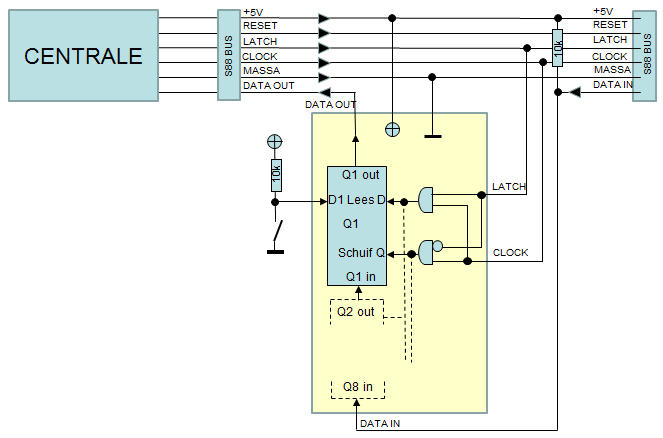
\includegraphics[width=0.8\textwidth]{./img/S88Bus.png}
		\caption{Schematische tekening van het S88 protocol.}

	\end{center}
\end{figure}


%http://users.telenet.be/RedDeBist/MBAAN/S88%20terugmelder.htm#S88 bus:
@online{ID,\\
	title = {S88 TERUGMELDERS},\\
	date = {04-03-2016},\\
	url = \url{http://users.telenet.be/RedDeBist/MBAAN/S88\%20terugmelder.htm}
		
	}
	
De rechter S88 bus zet paralelle data om naar seriele data, hoe dit gebeurt valt buiten de scope van dit onderzoek. Er wordt hier alleen onderzocht hoe een Xilinx bord met dit protocol kan communiceren.
\clearpage
	
\subsection{Hoe wordt het XILINX Spartan 3E FPGA bord gebruikt?}
%http://www.xilinx.com/support/documentation/data_sheets/ds312.pdf
Het FPGA bord krijgt instructies in de Hardware programeer taal VHDL om via het S88 protocol te controleren of er iets gebeurd op het RM88 bord. Dit houd in dat het FPGA bord een 'Clock' nodig heeft om te reageren op inkomende 'data' van het RM88 bord.\\
Dit wordt tot stand gebracht door op het FPGA bord via GPIO poorten verbinding te leggen naar het eerder vernoemde RM88 bord. To be continued